\section{Описание разработанных алгоритмов}
\label{sec:practice}


\subsection{Введение}

В предыдущей главе было рассказано об основных способах представления сигнала и базовых алгоритмах для работы с ним. Правильный подбор инструментов анализа играет решающую роль в успешном достижении цели. При обработке данных правильным образом сами собой становятся заметны особенности и закономерности, стоящие за ними. Тогда для принятия решения оказывается достаточно применения простых методов математической статистики.

В случае обнаружения сигналов ключевую роль играет частотно-временное представление. Оно сохраняет хронологию спектра, тем самым открывая для исследования изменение состава сигнала во времени. Оконное преобразование Фурье использовалось как предваряющий этап всех применяемых методов.

В общей постановке задача обнаружения сигналов очень сложна. Существует множество их типов и разновидностей помех. Можно назвать несколько важных характеристик, которые должен учитывать алгоритм: ширина полосы частот, модуляция, прерывается ли сигнал. Причем каждая их комбинация имеет право на жизнь. Пытаться покрыть все случаи сразу трудно и неэффективно. Разумнее разбить задачу на независимые части и решать их по отдельности.

Реальный тип сигнала всегда является причиной постановки новой подзадачи обнаружения. Не имеет смысла пытаться придумать решение абстрактной проблемы, ведь потом его придется исправлять под практические нужды. Каждый описанный алгоритм использует специфику встречающегося в эфире сигнала. Конечно, они могут сработать и с похожими на него, но изначально это не планировалось. Покрытие частных случаев может показаться слишком узкоспециализированным решением, но оно оправдывает себя. Во первых, большинство сигналов однотипны и для хорошего покрытия не требуется много алгоритмов. Во вторых, даже если удастся найти неопознанный сигнал, то возникает проблема его идентификации. Он может оказаться обычным шумом, каким-то образом прошедшим фильтрацию. А если это и не шум, то непонятно как извлечь из него информацию. В третьих, работа с частными случаями значительно упрощает алгоритмы и повышает доверие к ним. В четвертых, всегда можно добавить обобщенный обнаружитель, который будет иметь менее строгую фильтрацию. Его всегда можно использовать как запасной вариант.


\subsection{Архитектура}

Разработанный программный продукт представляет собой приложение для персонального компьютера, считывающее данные из заданного источника и выводящее на экран тип и полосу частот обнаруженных сигналов. Для взаимодействия с пользователем предусмотрен интерфейс командной строки. Реализация диктовалась требованиями, поставленными к конечному продукту. Вот основные из них:

\begin{itemize}
  \item{Способность считывать данные из различных источников (файл, радиоприемник и другие);}
  \item{Поддержка наиболее распространенных типов сигналов с возможностью добавлять новые;}
  \item{Работа в реальном времени;}
  \item{Оповещение о найденном сигнале с минимальной задержкой;}
  \item{Постоянный объем используемой памяти во времени.}
\end{itemize}

Возможность подменять источник данных оказывается очень полезной как при использовании, так и при разработке. Основным, конечно, является \SDR-приемник. Во время активности он непрерывно передает комплексные значения сигнала. Их нужно обработать как можно быстрее, чтобы успевать за потоком. Также эти значения можно сохранять в файл для последующего анализа. Поэтому нужен режим чтения из файла. В нем важно соблюдать ограничение по памяти --- комплексные семплы частотой более двух миллионов в секунду быстро образуют гигабайты информации. Обработать такой файл за один раз не получится. Помимо этих двух источников, предоставляющих реальные данные, для определения характеристик обнаружителя полезно проверять его на модельных сигналах. Они представляют собой функции уровня волны от времени и работают как на отдельных значениях, так и на их последовательности.

Очевидно, что столь разнородные источники стоит объединить общим интерфейсом. Им стал абстрактный \textbf{поставщик данных}. Его задача --- унификация доступа к данным, то есть определение эталонного образа делать это.

Предпочтительным оказался пакетный режим поставки. Он позволяет производить более эффективные операции над блоками данных и его можно реализовать во всех предполагаемых источниках. По команде "<старт"> поставщик начинает считывать данные, группировать их в блоки и при достижении заданного размера блока отправлять событие об его готовности. По команде "<стоп"> он досылает оставшиеся данные и прекращает свою работу.

Важно отметить использование событийной модели. Она обеспечивает слабую связность между компонентами системы. Заинтересованная сторона просто подписывается на событие поставщика. Она предоставляет функцию, которая выполнится, когда событие произойдет. Не требуется полагаться на детали реализации --- знать когда и откуда брать данные. Поставщику же не нужно следить, кому он должен их передать. Две стороны работают независимо, имея единственную точку соприкосновения. Это помогает и при отладке, когда можно легко вклиниться в цепочку обработки сигнала, не прерывая основной процесс.

В общем случае считывание данных из источника может быть блокирующей операцией. Это значит, что основной процесс приложения на это время полностью останавливается. Такое поведение значительно ухудшает общую производительность системы, поэтому считывание было вынесено в отдельный поток. Он запускается при старте поставщика данных, а при его остановке присоединяется к основному потоку.

Была упомянута польза работы с модельными данными. Реальные сигналы очень разнообразны, но над ними нет контроля --- можно экспериментировать только над теми, которые были вручную найдены и сохранены. Часто возникает желание проверить алгоритм на несколько модифицированном сигнале, чтобы убедиться в его обобщающей способности и узнать границы эффективного распознавания. В этом очень помогают математические модели. Любой сигнал в любой среде можно сымитировать. Конечно, эта имитация идеализирует реальные условия, но в целом достаточно хороша для исследовательских целей. Для решения этой задачи был реализован \textbf{микрофреймворк моделирования сигналов}.

Прежде всего он содержит примитивы, служащие строительными блоками для построения более сложных конструкций. К ним относятся волна с заданной амплитудой, частотой и начальной фазой и шум как случайный процесс с изменяемыми параметрами распределения. Далее возникает потребность комбинировать блоки. Это можно делать с помощью взвешенной суммы и поточечного умножения. Комбинация волн и шума дает различные по составу сигналы с аддитивными и мультипликативными помехами. Следующим шагом были реализованы основные методы модуляции. В совокупности с их помощью можно создавать сигналы близкие к реальным. Например, чтобы смоделировать зашумленный FM сигнал, содержащий синусоиду, нужно создать волну, FM-промодулировать ее и добавить аддитивный шум. Видны три ключевых шага: образование сигнала, представляющего полезную информацию, модуляция и добавление шума. Каждый из них можно модифицировать независимо от других, получая всевозможные виды сигналов.

API микрофреймворка моделирования сигналов представляет собой набор функций-конструкторов, реализующих описанные примитивы. Каждая из них возвращает функцию-замыкание, хранящую параметры модели. Их можно условно разделить на два типа: генераторы и комбинаторы. Генераторы оперируют над целыми числами, обозначающие моменты времени, либо над их массивами и возвращают комплексные значения уровня сигнала в это время. Комбинаторы принимают на вход один или более генераторов и, возможно, дополнительные параметры и возвращают новый генератор, являющийся продуктом объединения исходных.

Ниже приведен простейший пример моделирования синусоиды единичной амплитуды и частоты \SI{3.4}{\kilo\hertz}, FM-модулированной на несущей единичной амплитуды частотой \SI{80}{\mega\hertz}, с аддитивными помехами, представленными нормально распределенной случайной величиной с среднеквадратичным отклонением \num{0.5} (\autoref{lst:practice:modelling_example}).

\begin{listing}
  \begin{minted}{python}
    w = wave(A=1, f=3.4e3)
    nfm = fm(w, carrier_amp=1, carrier_freq=80e6, deviation=5)
    n = noise(std=0.5)
    noised_nfm = add(nfm, n)

    time = np.linspace(0, 1, 1000)
    signal = noised_nfm(time)
  \end{minted}
  \caption{Моделирование узкополосного FM сигнала}
  \label{lst:practice:modelling_example}
\end{listing}

Поставщик данных, работающий с моделями очень прост. При старте он инициализирует таймер нулевым значением, а затем "засыпает" на некоторое время. При следующей активации он рассчитывает, сколько прошло времени с последней активации, обновляет таймер и генерирует блок модельных данных за прошедший период времени с заданной частотой дискретизации.

Следующим звеном в цепи обработки сигнала является \textbf{сканер}. Его задача агрегировать поступающие данные, проводить их предобработку, отправлять на анализ и доводить до пользователя его результаты. Он работает на довольно абстрактном уровне, "склеивая" остальные части системы.

Для работы ему необходим поставщик данных, анализаторы и модуль ввода-вывода. Он подписывается на события, подаваемые поставщиком и накапливает приходящие данные. Когда их становится достаточно много, сканер выполняет над ними оконное преобразование Фурье и сохраняет его результаты в круговой буфер. Последний необходим из-за ограничения по памяти. Семплы приходят в очень большом объеме и хранить их все в памяти невозможно. Пару минут записи могут стать гигабайтами информации при большой частоте дискретизации. Поэтому приходится ограничиваться окном в несколько десятков секунд.

Таким образом, сканер всегда имеет частотно-временное представление сигнала в ближайшем временном интервале. При его обновлении инициируется событие, на которое подписаны анализаторы. Событийная модель предоставляет уже описанные преимущества --- слабая связность модулей и удобство отладки.

Для сканера анализаторы представляют собой "черные ящики". Он только инициирует событие и смотрит на результаты его обработки. Результаты --- это списки полос частот (возможно пустые), на которых анализаторы обнаружили сигнал. У сканера есть таблица частот, на которых уже были срабатывания. Он сопоставляет новые списки частот с этой таблицей и инициирует событие, на которое подписан модуль ввода-вывода. Он обновляет информацию на экране. Так текущее состояние системы отображается пользователю.

\textbf{Модуль ввода-вывода} очень прост. Он ожидает события сканера об обновлении списка частот и отображает его на экран. Возможно подменить модуль, работающий со стандартным потоком вывода в интерактивном режиме на модуль, пишущий в файл. Этот режим может быть использован для составления списка каналов, работающих в исследуемой полосе частот.

\textbf{Анализаторы} --- это основная рабочая сила приложения. Их задача принимать решения, на каких частотах наблюдаются нешумовые сигналы. Как было сказано, общую задачу обнаружения сигналов можно свести к набору частных задач обнаружения отдельных их типов. Поэтому для каждого поддерживаемого типа существует свой анализатор, который применяет специфичные алгоритмы.

Все анализаторы работают с частотно-временным представлением сигнала, но дальнейшая его обработка может сильно различаться. Они принимают на вход временное окно значений спектра и возвращают список частот обнаруженных сигналов. Такой общий интерфейс дает возможность применять их не завися от реализации.

Основной сценарий их использования --- обработка данных от радиоприемника в реальном времени. Это накладывает ограничения на вычислительную сложность используемых алгоритмов. Программное средство написано на языке \python, который не оптимален для тяжелых вычислений. На помощью приходит библиотека numpy, реализованная на языке \purec и интегрированная в \python как модуль. Она предоставляет средства для эффективных операций на матрицах, чем и являются частотно-временные представления сигнала. Распараллеливанием вычислений и использованием возможностей процессора по работе с гомогенными блоками данных, numpy удается достичь нескольких порядков прироста производительности в сравнении с чистым \python.

Для дальнейшей оптимизации можно применять различные эвристики. Например, скорость поступления новых данных зачастую избыточна для успешного обнаружения. Данные могут обновляться много раз в секунду. Такая детализация, конечно, повышает оперативность срабатывания обнаружителя, но практически не увеличивает достоверности его работы. Установка предельной частоты вызова анализаторов может повысить производительность практически без потерь эффективности.

На рисунке $TODO$ изображена общая архитектура системы. Прерывными линиями отмечено взаимодействие с использованием событий. Видно, что модули четко отделены друг от друга. Интерфейс между ними сведен к минимуму, требуется лишь уметь обрабатывать возникающие события и возвращать результаты в заданном формате. Это позволяет иметь совершенно различные в реализации модули и легко заменять их. Для функционирования необходим один поставщик данных, один сканер, один модуль ввода-вывода и один или более анализаторов. После их комбинирования запускается поставщик, который начинает генерировать данные. Сканер выполняет их предобработку и передает анализаторам, которые осуществляют решение. Затем он агрегирует полученные результаты и отправляет их к пользователю через модуль ввода-вывода.


\subsection{Анализатор широкополосных FM сигналов}

Широкополосные FM сигналы (WFM, Wideband FM) часто встречаются в радиоэфире.
В этом режиме работают коммерческие радиостанции.
Он хорош тем, что благодаря широкой полосе частот можно передать больший объем информации с более высокой четкостью. Это особенно важно при трансляции музыкальных произведений, которые содержат больше частот, чем обычный человеческий голос и для которых критична разборчивость приема. Широкий мощный сигнал доступен для воспроизведения бытовыми радиоприемниками.

\begin{figure}[h]
  \centering
  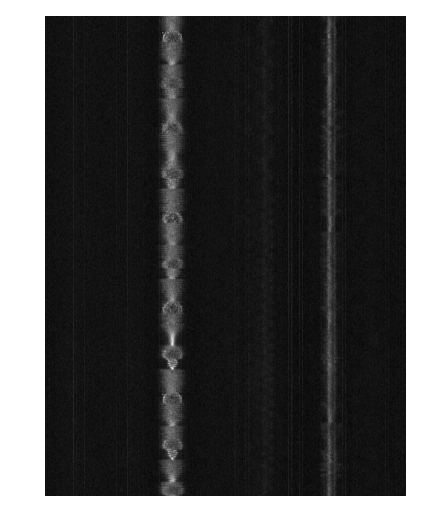
\includegraphics[height=0.6\textheight]{practice/wfm_spectrogram}
  \caption{Спектрограмма широкополосного FM сигнала}
  \label{fig:practice:wfm_spectrogram}
\end{figure}

К недостаткам в первую очередь можно отнести неэкономное использование частотного диапазона и большие затраты мощности на передачу сигнала. Это ограничивает его применение в основном небольшим количеством стационарных радиопередатчиков. Правда, радиус распространения волн диапазона, выделенного для WFM, невелик и в разных городах на близких частотах могут работать различные передатчики.

Обнаружить WFM сигнал достаточно просто. Как правило он не прерывается во времени и случайный процесс, описывающий его, имеет сравнительно стабильные параметры. Отсюда следует идея алгоритма --- искать частоты с активностью выше средней и выделять подходящие по ширине полосы. У широкополосного FM сигнала она может варьироваться в пределах \SIrange{100}{200}{\kilo\hertz}. Типичная для него спектрограмма изображена на рисунке \ref{fig:practice:wfm_spectrogram}. Очевидно выступает широкая полоса передачи радиостанции. Менее яркие линии --- это боковые лепестки.

Прежде всего необходимо определить уровень шума в исследуемом диапазоне частот. Зная это значение можно сразу же отфильтровать большую часть частот, на которых не наблюдается активности. Этот шаг с различными модификациями будет применяться во всех остальных алгоритмах из-за его вычислительной простоты и хорошей фильтрующей способности.

Измерять уровень шума можно по-разному. Самый простой способ --- это предопределить некоторый порог и считать все сигналы с меньшей мощностью шумовыми. Хотя такой подход и быстрее других, но его эффективность зависит от условий работы, коэффициента усиления приемника и других факторов. В зависимости от них возможно отфильтровывание настоящего сигнала и пропуск шума. Лучшей альтернативой было бы определять его мощность динамически всякий раз заново.

Напомним, что исследуется трехмерное представление --- время - частота - мощность. Произведем агрегацию по времени --- вычислим среднее значение. Получим среднюю мощность для каждой частоты. Такого результата можно было бы добиться применением обычного преобразования Фурье к полному временному ряду, но не всегда нужно именно среднее значение. Иногда лучше подходит, например, максимум, поэтому для общности алгоритмов эта оптимизация не была использована.

\begin{figure}[h]
  \centering
  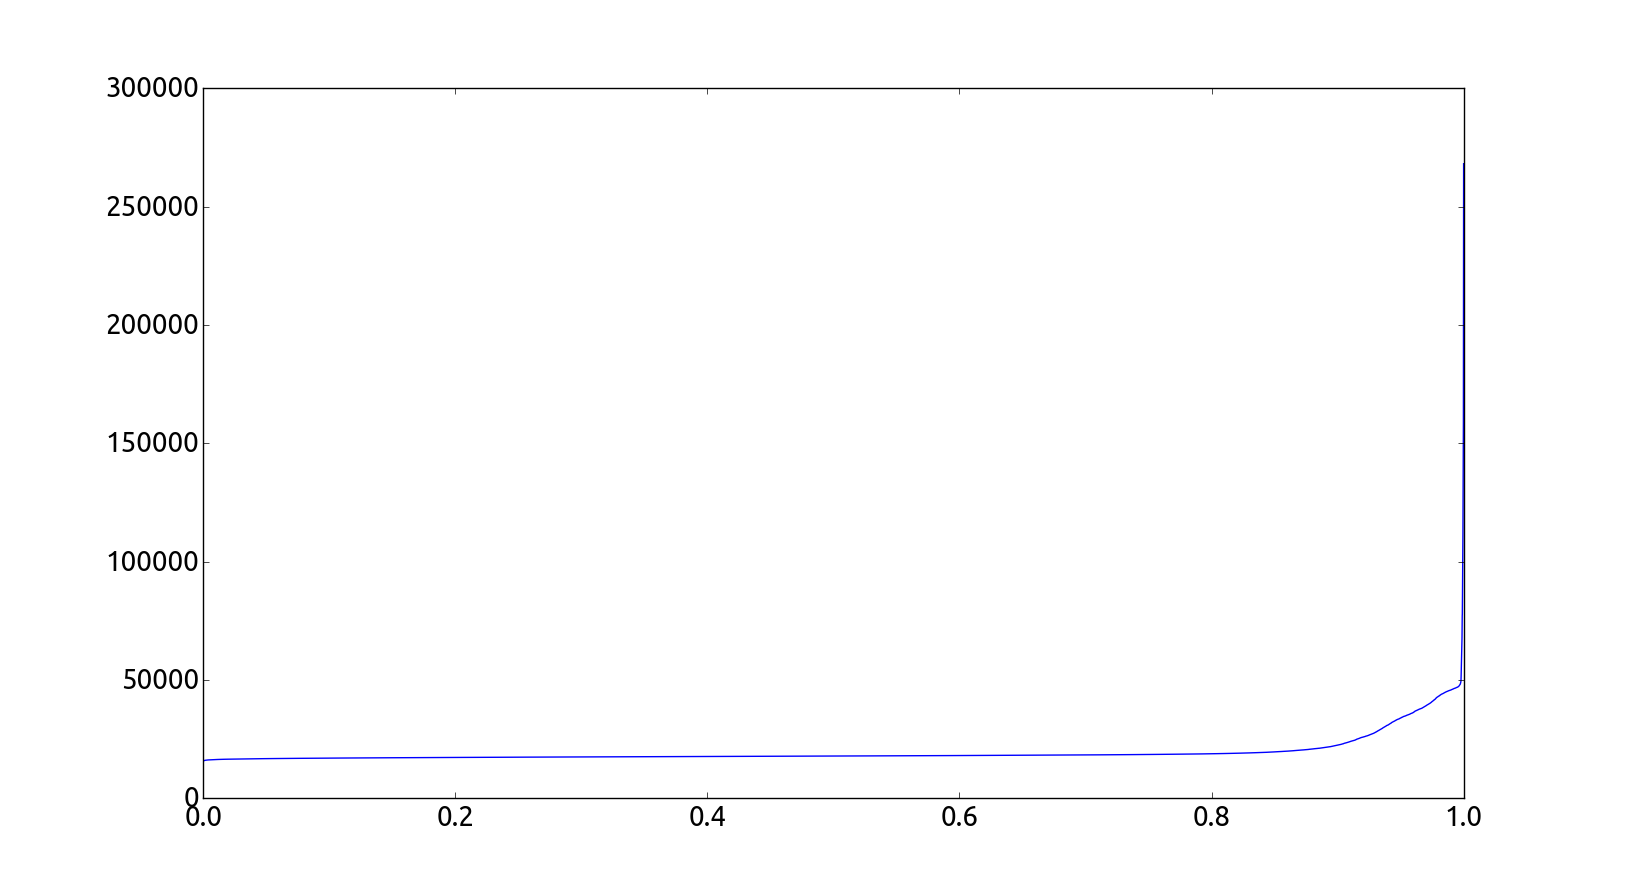
\includegraphics[width=0.9\textwidth]{practice/wfm_power_quantiles}
  \caption{Квантили распределения мощности сигнала}
  \label{fig:practice:wfm_power_quantiles}
\end{figure}

Теперь нужно понять, что считать шумом. В разных алгоритмах решение этой проблемы формулируется немного по разному. В случае WFM сигнала интересно некоторое среднее значение, которое с большой долей вероятности будет ниже значения сигнала, как в центре, так и на границах полосы. Если оно будет слишком большим, граничные значения отрежутся и сигнал потеряет свою оригинальную форму. Чтобы понять, как распределена мощность, полезно посмотреть на ее значения по квантилям (\autoref{fig:practice:wfm_power_quantiles}). Видно, что \SI{80}{\percent} частот содержат однородный шум и только около \SI{10}{\percent} что-то более выделяющееся. А пиковые значения наблюдаются лишь в \SI{1}{\percent} спектра. В данном случае за уровень шума можно выбрать любую квантиль ниже восьмедесятипроцентной, на этом интервале его мощность изменяется слабо. Для более общего случая подойдет значение \SI{60}{\percent}, чтобы гарантированно оставить информативные частоты.

Динамический квантильный подход значительно гибче выбора фиксированного порога, так как он адаптируется под каждую конкретную спектрограмму.

После выбора порога все частоты близкие к нему исключаются из дальнейшего рассмотрения. Такая фильтрация может создавать "пробелы" --- случайно исключенные частоты среди множества оставленных. Если их ширина меньше определенного порога, они возвращаются обратно, чтобы восстановить разорванные блоки.

Назовем эти блоки группами частот. Именно они в дальнейшем могут быть признаны каналами передачи информации. Для широкополосного FM сигнала тест очень прост --- ширина полосы частот группы должна лежать в допустимом интервале (\SIrange{100}{250}{\kilo\hertz}). Это условие оказывается достаточным на практике, так как шумовых сигналов такой ширины обычно не наблюдается и перепутать сигнал не с чем.

Повысить достоверность обнаружения можно, выполнив демодуляцию и проанализировав передаваемые данные. Если это не шум, будет наблюдаться вероятностное распределение близкое к нормальному. Но в реальности такие меры обычно избыточны и можно обойтись более простыми и вычислительно эффективными методами.


\subsection{Анализатор узкополосных FM сигналов}

Узкополосные FM сигналы (NFM, Narrowband FM) используются в качестве основного носителя в служебной связи.
Ценят их в первую очередь за эффективное использование частот. Каналы для них могут быть шириной всего \SI{10}{\kilo\hertz}. Конечно, столь малая девиация при FM модуляции позволяет более-менее отчетливо кодировать только узкий диапазон частот. Но в служебной связи достаточно передавать лишь основные составляющие человеческого голоса, чтобы речь была различимой, поэтому это ограничение не столь критично.

\begin{figure}[h]
  \centering
  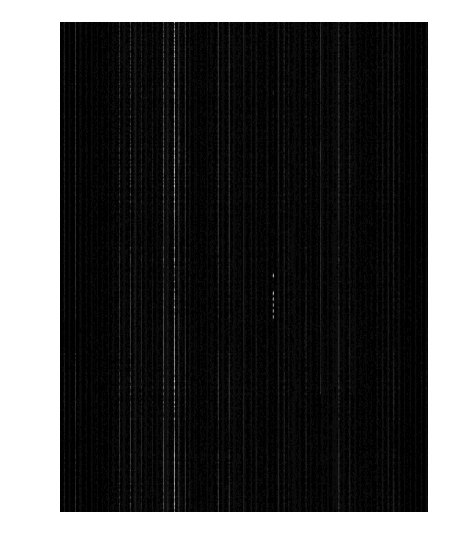
\includegraphics[height=0.6\textheight]{practice/nfm_spectrogram}
  \caption{Спектрограмма узкополосного FM сигнала}
  \label{fig:practice:nfm_spectrogram}
\end{figure}

Важной их особенностью является непостоянное присутствие в эфире. Обычно они проявляют себя только при активной передаче данных, а в остальное время канал пустует. Эта особенность настолько распространена, что говоря об узкополосных FM сигналах мы будем подразумевать ее наличие. Это не будет серьезным ограничением общности, так как даже если в периоды молчания подается некоторый однородный контрольный сигнал, разработанный алгоритм не потеряет своей эффективности.

В последние годы все большее распространение получает цифровая модуляция (манипуляция). Узкополосная частотная манипуляция --- наиболее часто применяющийся ее тип, не столь сильно отличается от NFM и может исследоваться теми же методами. Описываемый анализатор работает с обоими их разновидностями.

Типичный для NFM спектр изображен на рисунке \ref{fig:practice:nfm_spectrogram}. На нем наблюдаются периоды активности двух цифровых сигналов. То что они именно цифровые можно понять по прерывистой форме линий, состоящих, как-бы из отдельных маленьких кусочков. В случае аналогового сигнала эти линии были бы одним целым. Это различие не помешает распознаванию, так как алгоритм опирается не на форму линий, а на факт их появления и исчезновения.

Первый шаг предсказуем --- определение мощности шума и фильтрация шумовых частот. Особенность тут в том, что сигнал может быть кратковременным и усреднение по всему временному интервалу ухудшит его различимость. Поэтому вместо среднего вычисляется \SI{95}{\percent} квантиль. Она показывает, какой была близкая к максимальной мощность и не реагирует на ее случайные мгновенные всплески. Затем, как и в случае с WFM находится средняя мощность шума в спектре. Для каждой частоты эти два значения сравниваются. Если они близки, то частота исключается из рассмотрения как шумовая.

Придумать эвристику, способную отделять явный шум от информации несложно. Например, можно бинаризовать мощность по какому-то порогу, а затем посмотреть на группы нулей и единиц. Для сигнала они должны располагаться последовательными блоками. Тут возникает отличие между аналоговой и цифровой модуляцией --- в последнем случае блоки единиц (мощность выше пороговой) должны иметь примерно один размер и располагаться друг за другом с небольшими интервалами.

Другой более системный подход --- попробовать приблизить наблюдаемую последовательность математической моделью. Если модель, представляющая шум, будет давать неплохое приближение, то с большой долей уверенности можно считать последовательность шумовой.

Временные ряды можно моделировать с помощью $\ARMA$. В нашем случае это будет хронология значений мощности на фиксированной частоте. Полезный сигнал непредсказуем --- невозможно угадать, когда собеседник выйдет на связь и что он будет говорить в следующий момент. Поэтому можно предположить, что модель будет давать плохое приближение и это будет статистически заметно. Помехи же могут либо колебаться в районе каких-то значений, либо изменяться не слишком быстро, чтобы модель успевала подстроиться под изменение. В их случае приближение должно быть относительно хорошим, по крайней мере, оно должно четко отличаться от приближения полезной информации.

\begin{figure}[h]
  \centering
  \begin{subfigure}{0.45\textwidth}
    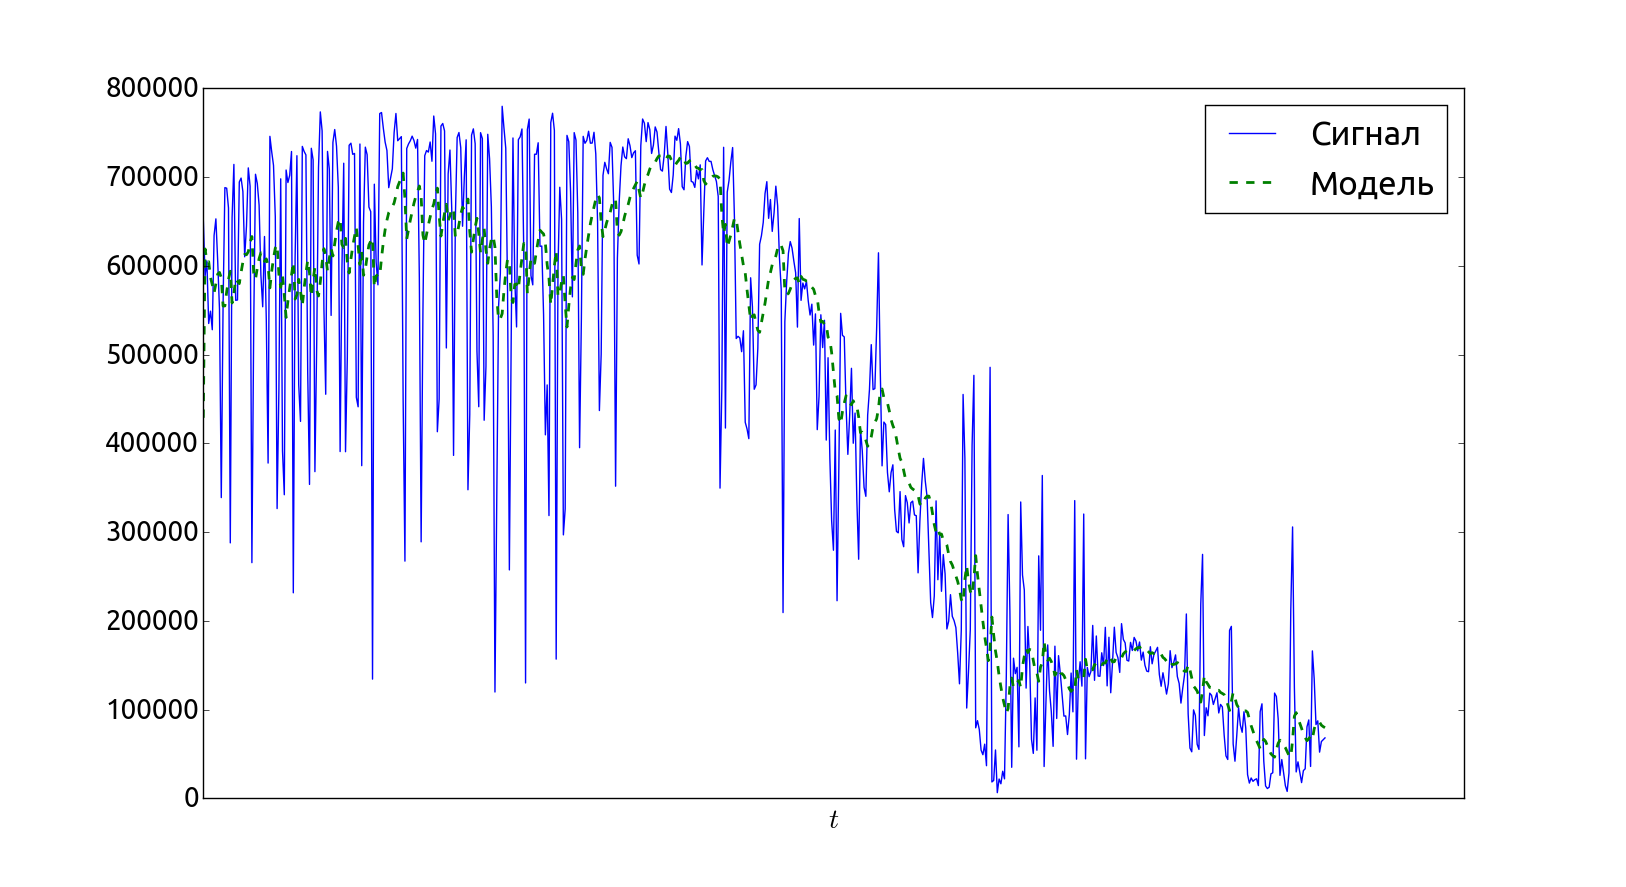
\includegraphics[width=\textwidth]{practice/arma_noise_approx}
    \caption{}
    \label{fig:practice:arma_noise_approx}
  \end{subfigure}
  \begin{subfigure}{0.45\textwidth}
    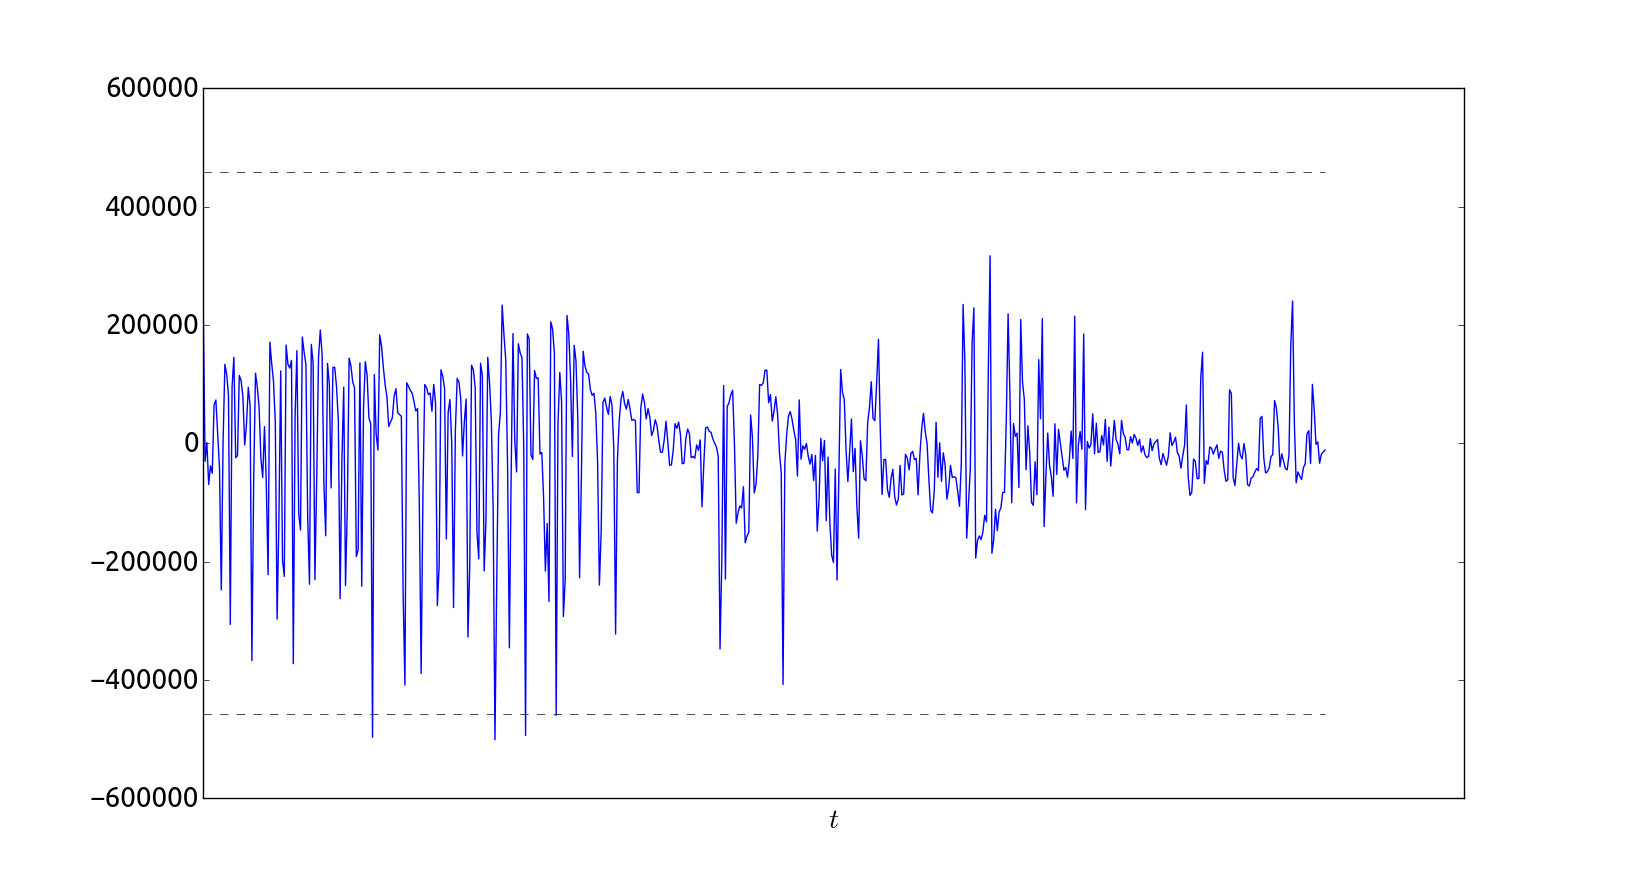
\includegraphics[width=\textwidth]{practice/arma_noise_resid}
    \caption{}
    \label{fig:practice:arma_noise_resid}
  \end{subfigure}
  \caption{Приближение моделью $\ARMA(1,1)$ на частоте, содержащей шум (\subref{fig:practice:arma_noise_approx}) и невязка приближения (\subref{fig:practice:arma_noise_resid}).}
  \label{fig:practice:arma_noise}
\end{figure}

На приведенной спектрограмме можно заметить тонкие полосы, тянущиеся сверху вниз. Это могут быть контрольные сигналы передатчиков или нечто другое, но для этого конкретного анализатора они не интересны. Выберем одну такую частоту и обучим на ней $\ARMA(1,1)$ (\autoref{fig:practice:arma_noise}). На рисунке \ref{fig:practice:arma_noise_approx} изображен график мощности от времени для реальных и модельных данных. Видно, что модель следует за общим трендом, но не отходит далеко от среднего. Это значит, что для минимизации ошибки она не рискует следовать за мгновенными изменениями ряда. Такое поведение характерно для непредсказуемой последовательности. Чтобы узнать о ней больше нужно проанализировать значения невязки.

Они изображены на соседнем рисунке \ref{fig:practice:arma_noise_resid}. Невязки достаточно большие и сравнимы с мощностью сигнала. Значит модель работает не очень хорошо. Это компенсируется адаптивным уровнем пределов, которые отмечены пунктиром. Все что выходит за них считается заслуживающим отдельного внимания. Хитрость в их выборе состоит в том, что они зависят от двух факторов: общего уровня шума на спектрограмме и мощности сигнала на рассматриваемой частоте. Первое нужно, чтобы не пропускать явно шумовые маломощные участки. Второе --- чтобы разрешать большие невязки на мощных сигналах, в данной работе оно принималось медианным значением.

Выбранные пределы пропускают лишь несколько мгновенных значений, которые будут отсеяны из-за недостаточной плотности и данная частота не будет включена в обнаруженные анализатором.

\begin{figure}[h]
  \centering
  \begin{subfigure}{0.45\textwidth}
    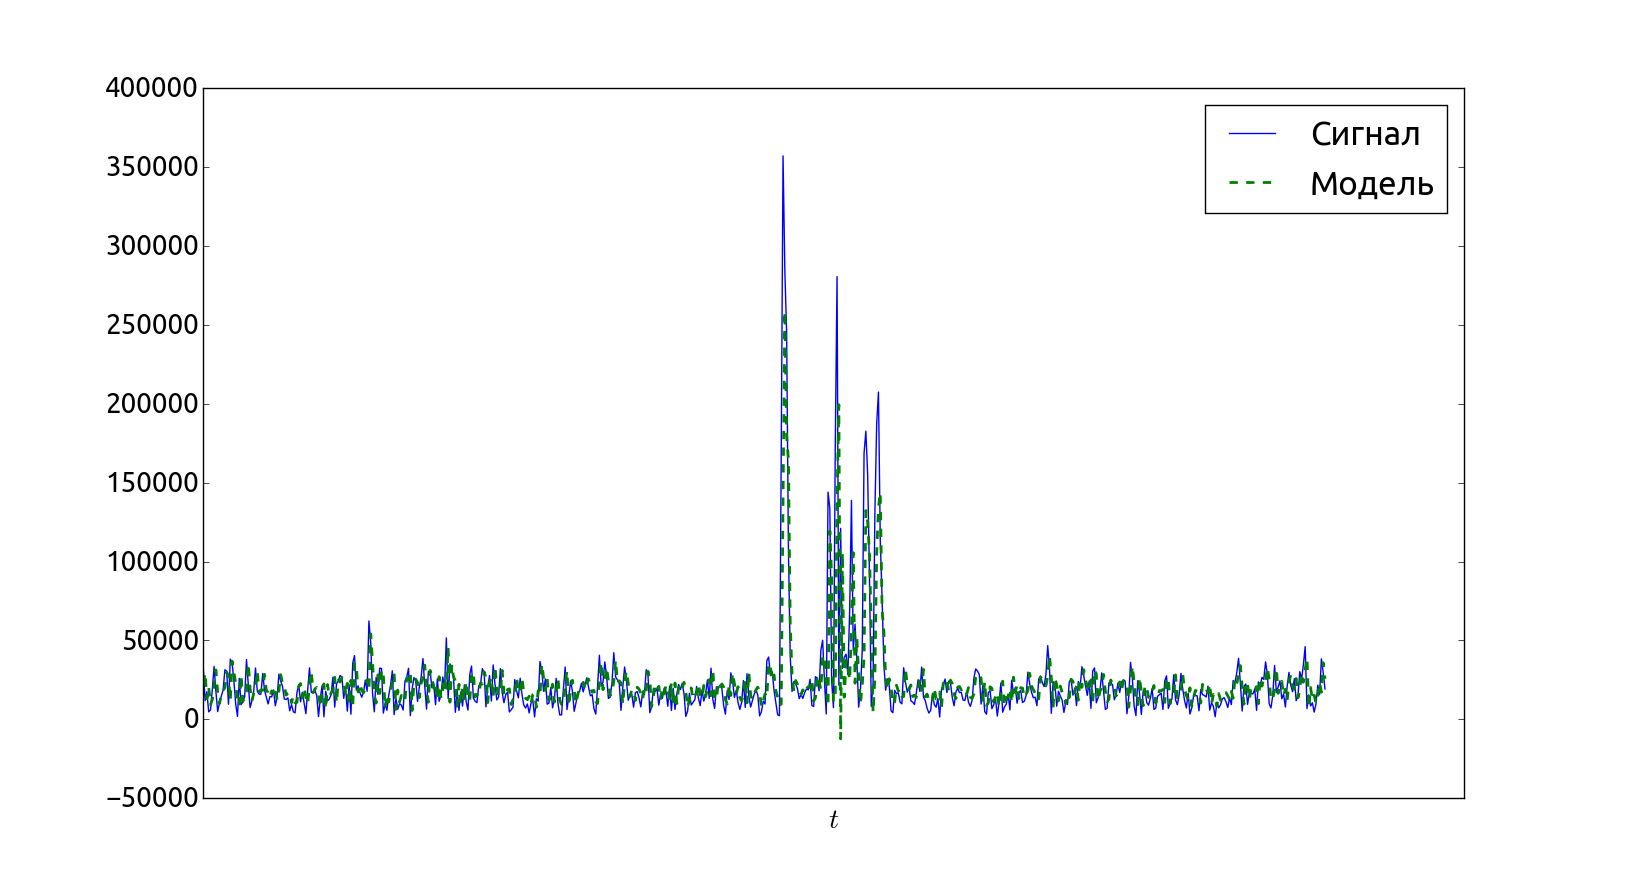
\includegraphics[width=\textwidth]{practice/arma_signal_approx}
    \caption{}
    \label{fig:practice:arma_signal_approx}
  \end{subfigure}
  \begin{subfigure}{0.45\textwidth}
    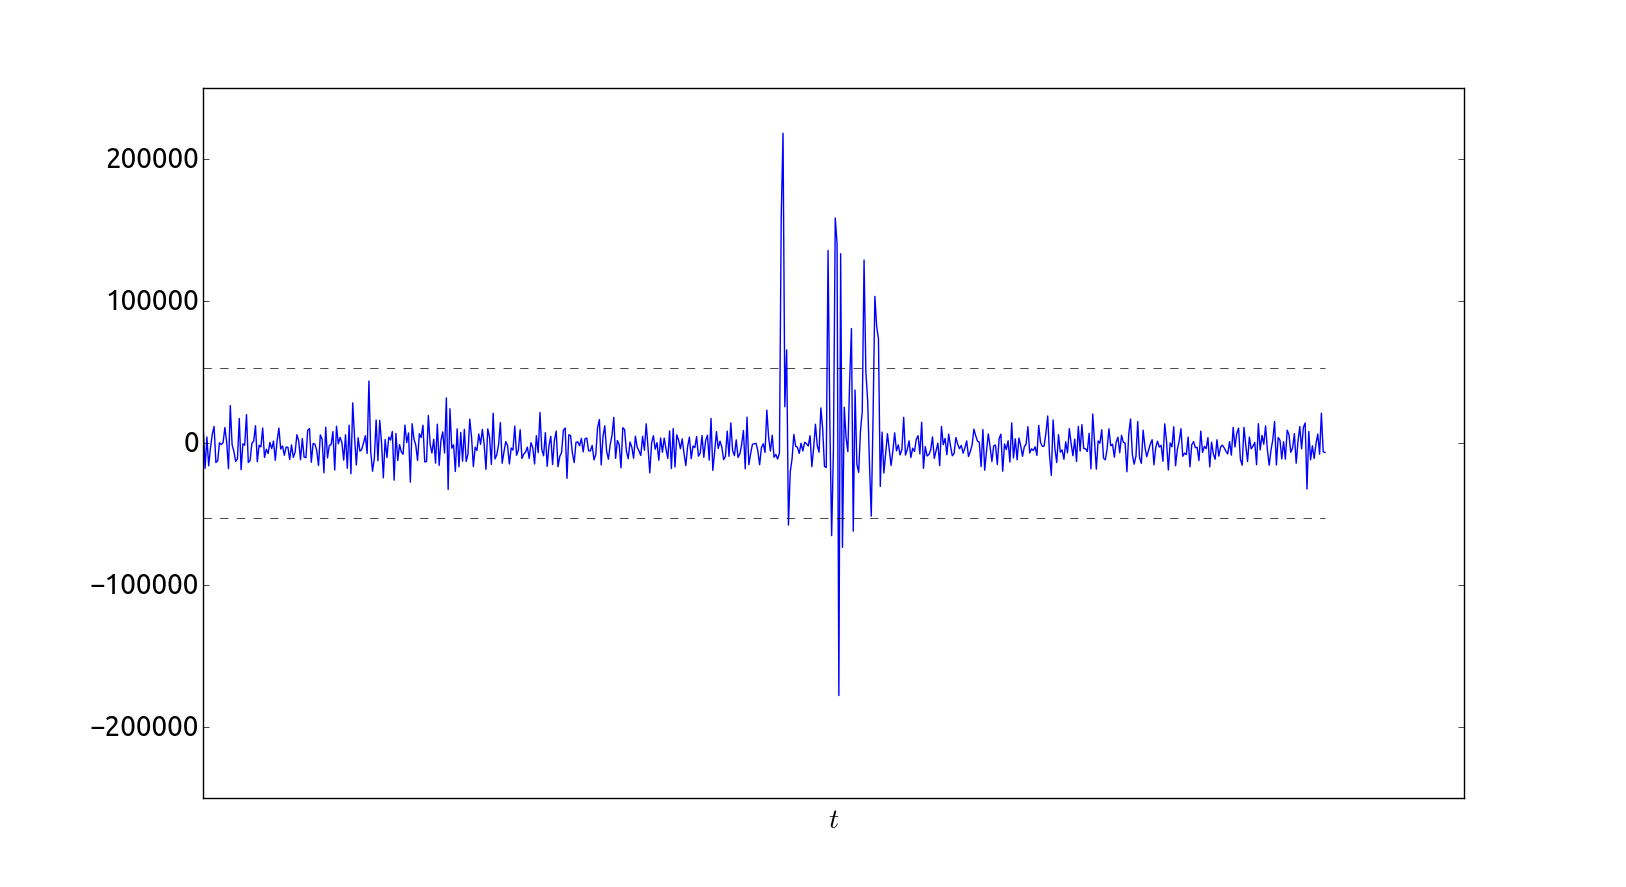
\includegraphics[width=\textwidth]{practice/arma_signal_resid}
    \caption{}
    \label{fig:practice:arma_signal_resid}
  \end{subfigure}
  \caption{Приближение моделью $\ARMA(1,1)$ на частоте, содержащей сигнал (\subref{fig:practice:arma_signal_approx}) и невязка приближения (\subref{fig:practice:arma_signal_resid}).}
  \label{fig:practice:arma_signal}
\end{figure}

Аналогичные графики, но уже для достоверного сигнала изображены на рисунке \ref{fig:practice:arma_signal}. На них отчетливо виден кратковременный всплеск мощности, соответствующий моменту передачи информации. Как и ожидалось, невязка модельных данных с истинными резко возрастает и выходит за установленные границы, которые здесь определены общим уровнем шума.

Плотность вышедших за границы значений сравнивается с некоторой заданной критической плотностью. Если она не была превышена, частота исключается из рассмотрения.

Оставшиеся частоты объединяются в группы, которые фильтруются по ширине (\SIrange{5}{50}{\kilo\hertz}). Прошедшие фильтрацию возвращаются как результат работы анализатора.

Таким образом, выделяются полосы частот, содержащие периодически появляющиеся NFM сигналы. У алгоритма есть одна особенность --- если частоты непрерывно используются, эффективность обнаружения может снижаться. Для них на этапе анализа невязок будут выставлены большие границы и невязки могут не выйти за них. Это ограничение не создает больших проблем на практике, так как даже если в канале происходит постоянная активность, она заканчивается и в этот момент гарантированно отлавливается алгоритмом. Более того, особенности сигналов с цифровой модуляцией обеспечивают достаточный для надежного обнаружения уровень "молчания". Такое решение было принято для достижения высокой специфичности анализатора --- он не срабатывает на многих непрерывных сигналах без явной активности.
